\chapter{Fragmenting Ping6 with NoAck}

In this chapter, in addition to compressing a ping6 request we will fragment it.
For that, we will create a ping6 request that exceeds the maximum L2 MTU allowed for the device:

~

\begin{termc}[backgroundcolor=\color{gray!10}, basicstyle=\ttfamily\small, escapechar=@]
ping6 -c 1 -s 200 2001:470:1f21:1d2::2
\end{termc}

\begin{lstlisting}[language=bash, basicstyle=\ttfamily\tiny, showstringspaces=false]
##[ IPv6 ]##
    version   = 6
    tc        = 0
    fl        = 63154
    plen      = 58
    nh        = ICMPv6
    hlim      = 52
    src       = 2001:41d0:302:2200::13b3
    dst       = 2001:470:1f21:1d2::2
##[ ICMPv6 Echo Request ]##
       type      = Echo Request
       code      = 0
       cksum     = 0xbc64
       id        = 0x260
       seq       = 0x1
       data      = '\\xa5\\xf3\x1cb\x00\x00\x00\x00\x9d\r\x00\x00\x00\x00\x00\x10\x1 1\x12\x13\x14\x15\x16\x17\x18
                    \x19\x1a\x1b\x1c\x1d\x1e\x1f!"#$%&\'()*+,-./0123456789:;<=>?@ABCDEFGHIJKLMNOPQRSTUVWXYZ[\\]^_`
                    abcdefghijklmnopqrstuvwxyz{|}~\x7f\\x80\\x81\\x82\\x83\\x84\\x85\\x86\\x87\\x88\\x89\\x8a\\x8b
                    \\x8c\\x8d\\x8e\\x8f\\x90\\x91\\x92\\x93\\x94\\x95\\x96\\x97\\x98\\x99\\x9a\\x9b\\x9c\\x9d\\x9e
                    \\x9f\\xa0\\xa1\\xa2\\xa3\\xa4\\xa5\\xa6\\xa7\\xa8\\xa9\\xaa\\xab\\xac\\xad\\xae\\xaf\\xb0\\xb1
                    \\xb2\\xb3\\xb4\\xb5\\xb6\\xb7\\xb8\\xb9\\xba\\xbb\\xbc\\xbd\\xbe\\xbf\\xc0\\xc1\\xc2\\xc3\\xc4
                    \\xc5\\xc6\\xc7''

    0000  FA 16 3E E9 DB 5D A2 C8 13 C9 D8 BC 08 00 45 00  ..>..]........E.
    0010  01 0C 79 DB 40 00 F0 29 33 33 D8 42 57 66 33 5B  ..y.@..)33.BWf3[
    0020  79 B6 60 00 F6 B2 00 D0 3A 34 20 01 41 D0 03 02  y.`.....:4 .A...
    0030  22 00 00 00 00 00 00 00 13 B3 20 01 04 70 1F 21  "......... ..p.!
    0040  01 D2 00 00 00 00 00 00 00 02 80 00 88 08 02 6B  ...............k
    0050  00 01 41 00 1D 62 00 00 00 00 14 3B 07 00 00 00  ..A..b.....;....
    0060  00 00 10 11 12 13 14 15 16 17 18 19 1A 1B 1C 1D  ................
    0070  1E 1F 20 21 22 23 24 25 26 27 28 29 2A 2B 2C 2D  .. !"#$%&'()*+,-
    0080  2E 2F 30 31 32 33 34 35 36 37 38 39 3A 3B 3C 3D  ./0123456789:;<=
    0090  3E 3F 40 41 42 43 44 45 46 47 48 49 4A 4B 4C 4D  >?@ABCDEFGHIJKLM
    00a0  4E 4F 50 51 52 53 54 55 56 57 58 59 5A 5B 5C 5D  NOPQRSTUVWXYZ[\]
    00b0  5E 5F 60 61 62 63 64 65 66 67 68 69 6A 6B 6C 6D  ^_`abcdefghijklm
    00c0  6E 6F 70 71 72 73 74 75 76 77 78 79 7A 7B 7C 7D  nopqrstuvwxyz{|}
    00d0  7E 7F 80 81 82 83 84 85 86 87 88 89 8A 8B 8C 8D  ~...............
    00e0  8E 8F 90 91 92 93 94 95 96 97 98 99 9A 9B 9C 9D  ................
    00f0  9E 9F A0 A1 A2 A3 A4 A5 A6 A7 A8 A9 AA AB AC AD  ................
    0100  AE AF B0 B1 B2 B3 B4 B5 B6 B7 B8 B9 BA BB BC BD  ................
    0110  BE BF C0 C1 C2 C3 C4 C5 C6 C7                    ..........
\end{lstlisting}

As one may notice, in this case the size of the \texttt{data} field of the ICMPv6 Echo Request is expanded in order to make the total package size larger. 
In this way, when the query arrives at the core it has to be first compressed and then fragmented so that it conforms to the MTU accepted by the device.

~

The following fragmentation rules are then added to the SoR and can be applied to that traffic:

\begin{lstlisting}[caption={Fragmentation Rules in rule icmp2.json}, backgroundcolor=\color{yellow}, basicstyle=\ttfamily\small, label=rule-icmp2]
	 },{
		"RuleID" : 12,
		"RuleIDLength" : 11,
		"Fragmentation" : {
			"FRMode": "NoAck",
			"FRDirection": "DW"
	 }
	 },{	
		"RuleID" : 13,
		"RuleIDLength" : 11,
		"Fragmentation" : {
		"FRMode": "NoAck",
		"FRDirection": "UP"
		} 
    }
]
}
\end{lstlisting}

\section{Understanding fragmentation rules}

In addition to the rule ID and the rule ID length a fragmentation rule contains two parameters: the mode and the direction.

~

In order to support reliability, variable L2 MTUs and unidirectional links, the RFC 8724 defines three different fragmentation modes: (i) No-Ack, designed for limited and variable MTU sizes under the assumption that there is no out-of-sequence delivery, (ii) Ack-on-Error for variable MTU and out-of-order delivery using sporadic ACK messages and (iii) Ack-allways for invariable MTUs and no out-of-sequence delivery.
In the following we will go deeper into details of these three modes.

~

As for the direction, it is necessary to stay the behaviour of the SCHC action based on where the traffic is originated.
In our example, we will use the rule \texttt{12/11} for fragmentation on Downlink and rule \texttt{13/11} for fragmentation on Uplink.
Therefore, if the traffic goes from the core to the device (Downlink), we use rule \texttt{12/11} for fragmenting the traffic at the core side and reassembling at the device side.
On the contrary, rule \texttt{13/11} is used for fragmenting the traffic going from the device to the co and for the reassembly processes at the core side.

~

As stated in RFC 8724, in OpenSCHC, SCHC Fragmentation is always done after compression\footnote{It shall rather be noted that, the no-compression rule is also permitted. Therefore, if one is willing to use only SCHC Fragmentation, two rules should be defined: (i) no-compression rule and (ii) the desired fragmentation rule.}. 
Then, as shown in Figure~\ref{fig-icmpv6_query} the whole process goes as following:

\begin{figure}[!tbp]
  \begin{minipage}[b]{0.33\columnwidth}
  \centering
    \usetikzlibrary{shadows,arrows.meta,positioning,backgrounds,fit}

\usetikzlibrary{shapes}
\usetikzlibrary{shapes.callouts}
\usetikzlibrary{shapes.geometric}

\usetikzlibrary{arrows}
\usetikzlibrary{decorations}
\usetikzlibrary{snakes}
\usetikzlibrary{calc}
\usetikzlibrary{patterns}

\usetikzlibrary{matrix,patterns,chains}
\usetikzlibrary{arrows,automata}
\usetikzlibrary{mindmap,trees}
\usetikzlibrary{shapes,snakes}
\usetikzlibrary{circuits.logic.US}
\usetikzlibrary{calc,intersections}

\tikzset{input/.style=coordinate}
\tikzset{output/.style=coordinate}
\tikzset{
  % coord node style is used for placing corners of connecting lines
  coord/.style={coordinate, on chain, on grid, node distance=6mm and 25mm},
  test/.style={draw, diamond, aspect=2, text width=5em},
  block/.style={draw, rectangle,
  minimum height=3em,
  minimum width=7em}}
  
\tikzset{pinstyle/.style={pin edge={to-,thin,black}}}

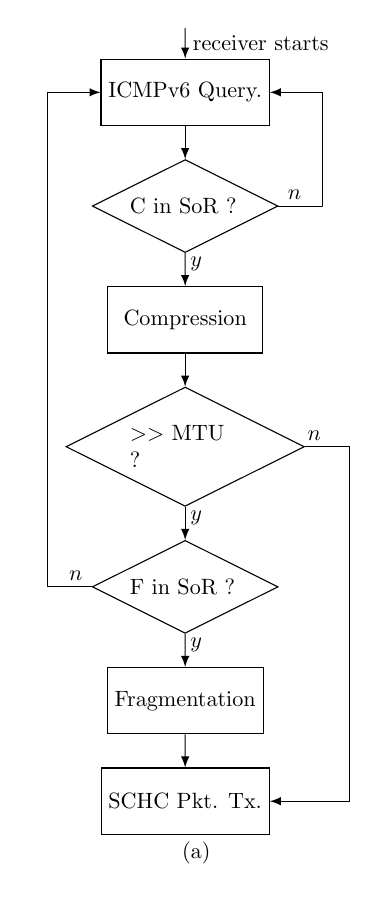
\begin{tikzpicture}[%auto, node distance=2cm,>=latex',
    xscale=0.8,
    yscale=0.8,
    transform shape,
    >=latex,              % Nice arrows; your taste may be different
    start chain=going below,    % General flow is top-to-bottom
    node distance=6mm and 60mm, % Global setup of box spacing
    every join/.style={norm},   % Default linetype for connecting boxes
    ]

\node (input) [input] {\textit{start}};

\node (start) [below right] at (input.south) {receiver starts};

\node (rx) [block, below, align=left] at (start.south west)
{ICMPv6 Query.};

\node (selectc) [test, below, align=left, yshift=-1.5em] at (rx.south)
{C in SoR ?};

\node [coord, right=of selectc] (non)  {}; %coordinates for the non path

\path (selectc.east) to node [near start, yshift = 0.5em] {$n$} (non); 
\path (selectc.south) to node [near start, xshift = 0.5em, yshift = -0.5em] {$y$} (selectc);

\node (comp) [block, below, align=left, yshift=-1.5em] at (selectc.south)
{Compression};

\node (selectmtu) [test, below, align=left, yshift=-1.5em] at (comp.south)
{$>>$ MTU ?};
\node [coord, right=of selectmtu] (non1)  {}; %coordinates for the non path
\path (selectmtu.east) to node [near start, yshift = 0.5em] {$n$} (non1); 
\path (selectmtu.south) to node [near start, xshift = 0.5em, yshift = -0.5em] {$y$} (selectmtu);

\node (selectf) [test, below, align=left, yshift=-1.5em] at (selectmtu.south)
{F in SoR ?};

\node [coord, left=of selectf] (non2)  {}; %coordinates for the non path
\path (selectf.west) to node [near start, yshift = 0.5em] {$n$} (non2); 
\path (selectf.south) to node [near start, xshift = 0.5em, yshift = -0.5em] {$y$} (selectf);


\node (frag) [block, below, align=left, yshift=-1.5em] at (selectf.south)
{Fragmentation};

\node (tx) [block, below, align=left, yshift=-1.5em] at (frag.south)
{SCHC Pkt. Tx.};

\draw [->] (input) --  (rx);    
\draw [->] (rx.south) -- (selectc);
\draw [->] (selectc.south) --  (comp);
\draw [->] (comp.south) --  (selectmtu);
\draw [->] (selectmtu.south) --  (selectf);
\draw [->] (selectf.south) --  (frag);
\draw [->] (frag.south) --  (tx);

\coordinate (fb) at ($(selectc.east)+(2em,0)$); %fb -- feedback
\draw [->] (selectc.east) -| (fb) |- (rx.east);

\coordinate (fb1) at ($(selectf.west)-(2em,0)$); %fb -- feedback
\draw [->] (selectf.west) -| (fb1) |- (rx.west);

\coordinate (fb) at ($(selectmtu.east)+(2em,0)$); %fb -- feedback
\draw [->] (selectmtu.east) -| (fb) |- (tx.east);

\path (tx.south) to node [near start, xshift = 0.5em, yshift = -0.8em] {(a)} (tx);


%\coordinate (fb) at ($(jam.west)+(-2em,0)$); %fb -- feedback
%\draw [->] (output) -| (fb) |- (loop.west);
%\coordinate (fb1) at ($(select.east)+(2em,0)$); %fb -- feedback
%\draw [->] (select.east) -| (fb1) |- (loop.east);

%\node (label) [below, yshift = - 0.3em] at (jam.south) {(a)};

\end{tikzpicture}
  \end{minipage}
  \hfill
  \begin{minipage}[b]{0.33\columnwidth}
  \centering
    \usetikzlibrary{shadows,arrows.meta,positioning,backgrounds,fit}

\usetikzlibrary{shapes}
\usetikzlibrary{shapes.callouts}
\usetikzlibrary{shapes.geometric}

\usetikzlibrary{arrows}
\usetikzlibrary{decorations}
\usetikzlibrary{snakes}
\usetikzlibrary{calc}
\usetikzlibrary{patterns}

\usetikzlibrary{matrix,patterns,chains}
\usetikzlibrary{arrows,automata}
\usetikzlibrary{mindmap,trees}
\usetikzlibrary{shapes,snakes}
\usetikzlibrary{circuits.logic.US}
\usetikzlibrary{calc,intersections}

\tikzset{input/.style=coordinate}
\tikzset{output/.style=coordinate}
\tikzset{
  % coord node style is used for placing corners of connecting lines
  coord/.style={coordinate, on chain, on grid, node distance=6mm and 25mm},
  test/.style={draw, diamond, aspect=2, text width=5em},
  block/.style={draw, rectangle,
  minimum height=3em,
  minimum width=7em}}
  
\tikzset{pinstyle/.style={pin edge={to-,thin,black}}}

\begin{tikzpicture}[%auto, node distance=2cm,>=latex',
    xscale=0.8,
    yscale=0.8,
    transform shape,
    >=latex,              % Nice arrows; your taste may be different
    start chain=going below,    % General flow is top-to-bottom
    node distance=6mm and 60mm, % Global setup of box spacing
    every join/.style={norm},   % Default linetype for connecting boxes
    ]

\node (input) [input] {\textit{start}};

\node (start) [below right] at (input.south) {transmitter starts};

\node (rx) [block, below, align=left] at (start.south west)
{SCHC Pkt Rx.};

\node (selectf) [test, below, align=left, yshift=-1.5em] at (rx.south)
{F in SoR ?};

\node [coord, right=of selectf] (non)  {}; %coordinates for the non path

\path (selectf.west) to node [near start, yshift = 0.5em, xshift = -3em] {$n$} (non); 
\path (selectf.south) to node [near start, xshift = 0.5em, yshift = -0.5em] {$y$} (selectf);

\node (reas) [block, below, align=left, yshift=-1.5em] at (selectf.south)
{Reassembly};

\node (selectc) [test, below, align=left, yshift=-1.5em] at (reas.south)
{C in SoR ?};
\node [coord, right=of selectc] (non)  {}; %coordinates for the non path
\path (selectc.east) to node [near start, yshift = 0.5em] {$n$} (non1); 
\path (selectc.south) to node [near start, xshift = 0.5em, yshift = -0.5em] {$y$} (selectc);


\node (decomp) [block, below, align=left, yshift=-1.5em] at (selectc.south)
{Decompression};

\node [coord, right=of decomp] (non1)  {}; %coordinates for the non path


\node (query) [block, below, align=left, yshift=-1.5em] at (decomp.south)
{ICMPv6 Query};

\node (resp) [block, below, align=left, yshift=-1.5em] at (query.south)
{Echo App.};

\draw [->] (input) --  (rx);    
\draw [->] (rx.south) -- (selectf);
\draw [->] (selectf.south) --  (reas);
\draw [->] (reas.south) --  (selectc);
\draw [->] (selectc.south) --  (decomp);
\draw [->] (decomp.south) --  (query);
\draw [->] (query.south) --  (resp);

\coordinate (fb) at ($(selectf.west)-(2em,0)$); %fb -- feedback
\draw [->] (selectf.west) -| (fb) |- (selectc.west);

\coordinate (fb1) at ($(selectc.east)+(2em,0)$); %fb -- feedback
\draw [->] (selectc.east) -| (fb1) |- (rx.east);

\node (label) [below, yshift = - 0.3em] at (resp.south) {(b)};

\end{tikzpicture}

  \end{minipage}
\caption{ICMPv6 Query Reception when MTU exceeds L2 MTU: (a) Receiver behaviour, (b) Transmitter behaviour.} \label{fig-icmpv6_query}
\end{figure}

\begin{itemize}
    \item ICMPv6 Echo Request Query Reception at core (Figure.\ref{fig-icmpv6_query}(a))
\begin{enumerate}
    \item An user send a ICMPv6 Echo request exceeding the maximum MTU allowed.
    \item The request arrives at the core side. It verifies if there is a compression rule on its SoR applicable to this specific traffic.
    \item If it exists, the core applies the compression rule. 
    Then, it verifies if the resulting packet surpasses the L2 MTU size.
    \item If yes, the core verifies if there is a fragmentation rule on dowlink.
    \item If there is one, the core applies the fragmentation using the mode defined in the rule.
    \item The core starts to send fragments to the device.
    \end{enumerate}

\item ICMPv6 Echo Request Query Reception at device (Figure.\ref{fig:icmpv6_query}(b)) : 
\begin{enumerate}
    \item The device receives SCHC packets containing the fragments.
    \item The device verifies if there is a fragmentation rule and start the reassembly process.
    \item Once the reassembly process is finished, the device search for a compression ruls applicable to this specific traffic.
    \item The device applies the compression rule to decompress the packet.
    \item The device retrieves the ICMPv6 Echo Reply Query.
    \item At the application level, the device creates a ICMPv6 Echo Reply.
\end{enumerate}

\item ICMPv6 Echo Reply Query Transmission at device (Figure.\ref{fig:icmpv6_query}(a)) : 
\begin{enumerate}
    \item The device verifies if there is a Compression rule for the ICMPv6 Echo Reply.
    \item If yes, the device compress the packet.
    \item The device verifies if the resulting packet surpasses the L2 MTU size.
    \item If yes, it looks for a Fragmentation rule in its SoR applicable to this traffic.
    \item If there is one, the device applies the fragmentation using the mode as defined in the rule.
    \item The device start to send fragments to the device.
\end{enumerate}

\item ICMPv6 Echo Reply Query Reception at core (Figure.\ref{fig:icmpv6_query}(b)) : 
\begin{enumerate}
    \item The core receives SCHC packets containing the fragments.
    \item The core verifies if there is fragmentation rule in its SoR, if yes, it starts the reassembly process.
    \item Once finished, the core search for compression rules applicable to this specific traffic 
    \item If there is a compression rue, it decompress the packet.
    \item The core forwards the ICMPv6 Echo Reply to the user.
\end{enumerate}
\end{itemize}

\section{Fragmentation in No-ACK mode}

This fragmentation mode is designed for no out-of sequence delivery and admits variable L2 MTU.
In No-ACK mode, there is no communication from the fragment receiver to the fragment sender.  
The sender transmits all the SCHC Fragments without expecting any acknowledgement.  
Therefore, there is no need for bidirectional links.

\subsection{SCHC Fragments Format}

In No-ACK, there are two kinds of SCHC Fragments: (i) \texttt{All-0} fragments presented in Figure.\ref{fig-all-0}, and the last fragment called \texttt{All-1} depicted in Figure.\ref{fig-all-1}
An all-0 fragment, is composed of the following fields\footnote{The RFC 8724 also defines the \texttt{DTag} (Datagram Tag) and the \texttt{W} (Window) fields. The former is used for differentiating SCHC F/R messages belonging to different SCHC Packets, for our example this field is not present, and the latter, representing the Window size used in Ack-on-Error and Ack-Allways modes}:

~

\begin{itemize}
    \item \texttt{RuleID}
    %\item W:
    \item \texttt{FCN}: It is used to differentiate All-0 and All-1 fragments. 
    \item \texttt{Fragment Payload}: Corresponds to the payload. Its size is aligned to the remaining space from to fit the L2 MTU.
\end{itemize}

~

\begin{figure}[!ht] 
    \centering 
    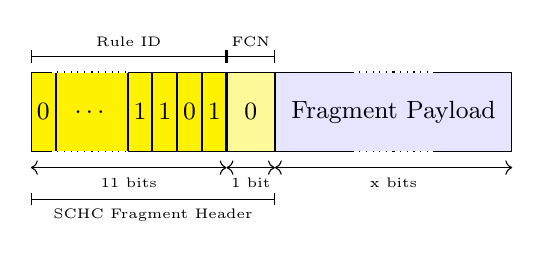
\begin{tikzpicture}

\draw (0,0) node (b1)  [rectangle, draw, minimum height=1cm, minimum width = 0.3cm, fill=yellow] {};
\draw(b1) node {\small{0}};
\draw (b1.east) node (b2)  [right, rectangle, draw, minimum height=1cm, minimum width = 0.9cm, fill=yellow] {};
\draw(b2) node {\small{\dots}};


\draw [white, thick] (b2.north) -- +(0.5, 0);
\draw [white, thick] (b2.north) -- +(-0.5, 0);

\draw [dotted] (b2.north) -- +(0.5, 0);
\draw [dotted] (b2.north) -- +(-0.5, 0);

\draw [white, thick] (b2.south) -- +(0.5, 0);
\draw [white, thick] (b2.south) -- +(-0.5, 0);

\draw [dotted] (b2.south) -- +(0.5, 0);
\draw [dotted] (b2.south) -- +(-0.5, 0);


\draw (b2.east) node (b8)  [right, rectangle, draw, minimum height=1cm, minimum width = 0.3cm, fill=yellow] {};
\draw(b8) node {\small{1}};

\draw (b8.east) node (b9)  [right, rectangle, draw, minimum height=1cm, minimum width = 0.3cm, fill=yellow] {};
\draw(b9) node {\small{1}};

\draw (b9.east) node (b10)  [right, rectangle, draw, minimum height=1cm, minimum width = 0.3cm, fill=yellow] {};
\draw(b10) node {\small{0}};

\draw (b10.east) node (b11)  [right, rectangle, draw, minimum height=1cm, minimum width = 0.3cm, fill=yellow] {};
\draw(b11) node {\small{1}};
\path(b1.north) -- +(0, 0.2) coordinate(hlineu);

\draw [|-|] (b1.west |- hlineu) -- coordinate(a) (b11.east |- hlineu) ;
\draw (a) node [above] {\tiny{Rule ID}};
\path(b1.south) -- +(0, -0.2) coordinate(hline);

\draw [<->] (b1.west |- hline) -- coordinate(a) (b11.east |- hline) ;
\draw (a) node [below] {\tiny{11 bits}};
\draw (b11.east) node (dtag) [right, rectangle, draw, minimum height=1cm, minimum width=1cm, fill=yellow!30]{};
%\draw (dtag) node {\small{DTag}};
%\path(b1.south) -- +(0, -0.2) coordinate(hline);


%\path(b1.south) -- +(0, -0.2) coordinate(hline);
%\draw [<->] (dtag.west |- hline) -- coordinate(a) (dtag.east |- hline) ;
%\draw (a) node [below] {\tiny{T bits}};


\draw (b11.east) node (fcn) [right, rectangle, draw, minimum height=1cm, minimum width=0.6cm, fill=yellow!40]{};
\draw (fcn.text) node {\small{0}};

\draw [|-|] (fcn.west |- hlineu) -- coordinate(a) (fcn.east |- hlineu) ;
\draw (a) node [above] {\tiny{FCN}};
\path(b1.south) -- +(0, -0.2) coordinate(hline);

\draw [<->] (fcn.west |- hline) -- coordinate(a) (fcn.east |- hline) ;
\draw (a) node [below] {\tiny{1 bit}};

%\draw (fcn.east) node (rcs) [right, rectangle, draw, minimum height=1cm, minimum width=1cm, fill=green!10]{};
%\draw (rcs.text) node {\small{RCS}};

%\draw [<->] (rcs.west |- hline) -- coordinate(a) (rcs.east |- hline) ;
%\draw (a) node [below] {\tiny{32 bits}};

\draw (fcn.east) node (fpay) [right, rectangle, draw, minimum height=1cm, minimum width=3cm, fill=blue!10]{};
\draw (fpay.text) node {\small{Fragment Payload}};

\draw [white, thick] (fpay.north) -- +(0.5, 0);
\draw [white, thick] (fpay.north) -- +(-0.5, 0);
\draw [dotted] (fpay.north) -- +(0.5, 0);
\draw [dotted] (fpay.north) -- +(-0.5, 0);

\draw [white, thick] (fpay.south) -- +(0.5, 0);
\draw [white, thick] (fpay.south) -- +(-0.5, 0);
\draw [dotted] (fpay.south) -- +(0.5, 0);
\draw [dotted] (fpay.south) -- +(-0.5, 0);

\draw [<->] (fpay.west |- hline) -- coordinate(a) (fpay.east |- hline) ;
\draw (a) node [below] {\tiny{x bits}};

\path(b1.south) -- +(0, - 0.6) coordinate(hline1);
\draw [|-|] (b1.west |- hline1) -- coordinate(a) (fcn.east |- hline1) ;
coordinate 
\draw (a) node [below] {\tiny{SCHC Fragment Header}};

\end{tikzpicture}
    \caption{All-0 SCHC Fragment in No-Ack mode} 
    \label{fig-all-0} 
\end{figure} 

The second type of fragment is the \texttt{All-1}, it corresponds to the last fragment. As shown in Figure \ref{fig:all-1}, contrary to the \texttt{All-0}, it also contains the RCS field, and it can also contains padding as needed in order to fit the L2 word size.

\begin{figure}[!ht] 
    \centering 
    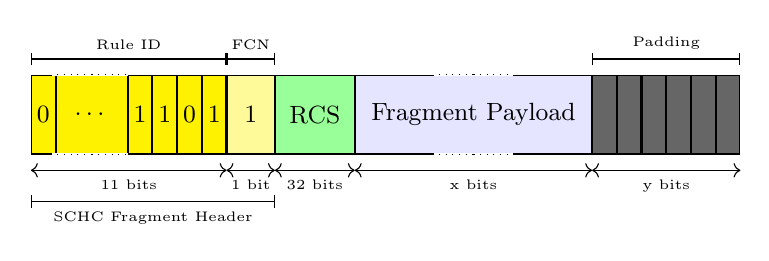
\begin{tikzpicture}

\draw (0,0) node (b1)  [rectangle, draw, minimum height=1cm, minimum width = 0.3cm, fill=yellow] {};
\draw(b1) node {\small{0}};
\draw (b1.east) node (b2)  [right, rectangle, draw, minimum height=1cm, minimum width = 0.9cm, fill=yellow] {};
\draw(b2) node {\small{\dots}};


\draw [white, thick] (b2.north) -- +(0.5, 0);
\draw [white, thick] (b2.north) -- +(-0.5, 0);

\draw [dotted] (b2.north) -- +(0.5, 0);
\draw [dotted] (b2.north) -- +(-0.5, 0);

\draw [white, thick] (b2.south) -- +(0.5, 0);
\draw [white, thick] (b2.south) -- +(-0.5, 0);

\draw [dotted] (b2.south) -- +(0.5, 0);
\draw [dotted] (b2.south) -- +(-0.5, 0);


\draw (b2.east) node (b8)  [right, rectangle, draw, minimum height=1cm, minimum width = 0.3cm, fill=yellow] {};
\draw(b8) node {\small{1}};

\draw (b8.east) node (b9)  [right, rectangle, draw, minimum height=1cm, minimum width = 0.3cm, fill=yellow] {};
\draw(b9) node {\small{1}};

\draw (b9.east) node (b10)  [right, rectangle, draw, minimum height=1cm, minimum width = 0.3cm, fill=yellow] {};
\draw(b10) node {\small{0}};

\draw (b10.east) node (b11)  [right, rectangle, draw, minimum height=1cm, minimum width = 0.3cm, fill=yellow] {};
\draw(b11) node {\small{1}};
\path(b1.north) -- +(0, 0.2) coordinate(hlineu);

\draw [|-|] (b1.west |- hlineu) -- coordinate(a) (b11.east |- hlineu) ;
\draw (a) node [above] {\tiny{Rule ID}};
\path(b1.south) -- +(0, -0.2) coordinate(hline);

\draw [<->] (b1.west |- hline) -- coordinate(a) (b11.east |- hline) ;
\draw (a) node [below] {\tiny{11 bits}};

\draw (b11.east) node (fcn) [right, rectangle, draw, minimum height=1.0cm, minimum width=0.6cm, fill=yellow!40]{};
\draw (fcn) node {\small{1}};

\draw [|-|] (fcn.west |- hlineu) -- coordinate(a) (fcn.east |- hlineu) ;
\draw (a) node [above] {\tiny{FCN}};
\path(b1.south) -- +(0, -0.2) coordinate(hline);

\draw [<->] (fcn.west |- hline) -- coordinate(a) (fcn.east |- hline) ;
\draw (a) node [below] {\tiny{1 bit}};

\draw (fcn.east) node (rcs) [right, rectangle, draw, minimum height=1cm, minimum width=1cm, fill=green!40]{};
\draw (rcs.text) node {\small{RCS}};

\draw [<->] (rcs.west |- hline) -- coordinate(a) (rcs.east |- hline) ;
\draw (a) node [below] {\tiny{32 bits}};

\draw (rcs.east) node (fpay) [right, rectangle, draw, minimum height=1cm, minimum width=3cm, fill=blue!10]{};
\draw (fpay.text) node {\small{Fragment Payload}};

\draw [white, thick] (fpay.north) -- +(0.5, 0);
\draw [white, thick] (fpay.north) -- +(-0.5, 0);
\draw [dotted] (fpay.north) -- +(0.5, 0);
\draw [dotted] (fpay.north) -- +(-0.5, 0);

\draw [white, thick] (fpay.south) -- +(0.5, 0);
\draw [white, thick] (fpay.south) -- +(-0.5, 0);
\draw [dotted] (fpay.south) -- +(0.5, 0);
\draw [dotted] (fpay.south) -- +(-0.5, 0);

\draw [<->] (fpay.west |- hline) -- coordinate(a) (fpay.east |- hline) ;
\draw (a) node [below] {\tiny{x bits}};

\draw (fpay.east) node (p1)  [right, rectangle, draw, minimum height=1cm, minimum width = 0.3cm, fill=black!60] {};
\draw (p1.east) node (p2)  [right, rectangle, draw, minimum height=1cm, minimum width = 0.3cm, fill=black!60] {};
\draw (p2.east) node (p3)  [right,rectangle, draw, minimum height=1cm, minimum width = 0.3cm, fill=black!60] {};
\draw (p3.east) node (p4)  [right,rectangle, draw, minimum height=1cm, minimum width = 0.3cm, fill=black!60] {};
\draw (p4.east) node (p5)  [right,rectangle, draw, minimum height=1cm, minimum width = 0.3cm, fill=black!60] {};
\draw (p5.east) node (p6)  [right,rectangle, draw, minimum height=1cm, minimum width = 0.3cm, fill=black!60] {};

\path(b1.south) -- +(0, - 0.6) coordinate(hline1);
\draw [|-|] (b1.west |- hline1) -- coordinate(a) (fcn.east |- hline1) ;
coordinate 
\draw (a) node [below] {\tiny{SCHC Fragment Header}};


\draw [|-|] (p1.west |- hlineu) -- coordinate(a) (p6.east |- hlineu) ;
\draw (a) node [above] {\tiny{Padding}};

\draw [<->] (p1.west |- hline) -- coordinate(a) (p6.east |- hline) ;
\draw (a) node [below] {\tiny{y bits}};

\end{tikzpicture}

    \caption{All-1 SCHC Fragment in No-Ack mode} 
    \label{fig-all-1} 
\end{figure} 
   
In OpenSCHC the Reassembly Check Sequence (RCS) field corresponds to the result of using the CRC32 algorithm, and as recommended by the RFC 8724 it is computed on the full SCHC packet (after reassembly) concatenated with the padding bits.

\subsection{Fragmentation/Reassembly Process}

In this mode, since there are no fragment acknowledgments, the sender creates as many fragments as needed based on the size of the compressed SCHC packet and the L2 MTU.
Figure \ref{fig-NoAck} presents an example where $n$ fragments are needed. 
In this case, the transmitter creates $n-1$ \texttt{All-0} fragments and one \texttt{All-1} with the corresponding RCS field and padding if needed.

\begin{figure}[!ht] 
    \centering 
    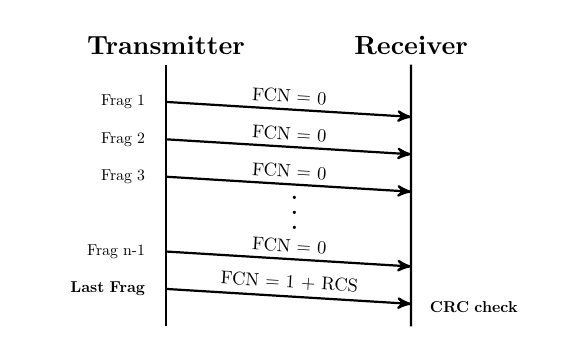
\begin{tikzpicture}[xscale = 0.95, yscale = 0.95,transform shape,>=stealth',thick,
commentl/.style={text width=2.5cm, align=right, scale=.6},
commentr/.style={commentl, align=left}]

\node[] (init) {\textbf{Transmitter}};
\node[right=1.2cm of init] (core) {\textbf{Receiver}};
\node[right=0.4cm of init] (middle) {};

\draw[->] ([yshift=-0.5cm]init.south) coordinate (f1) -- ([yshift=-.2cm]f1-|core)
coordinate (fin1) node[pos=.5, above, sloped, scale=0.7] {FCN = 0};
\node[left = 2mm of f1.west, commentl]{Frag 1};

\draw[->] ([yshift=-1cm]init.south) coordinate (f2) -- ([yshift=-.7cm]f1-|core)
coordinate (fin2) node[pos=.5, above, sloped, scale=0.7] {FCN = 0};
\node[left = 2mm of f2.west, commentl]{Frag 2};

\draw[->] ([yshift=-1.5cm]init.south) coordinate (f3) -- ([yshift=-1.2cm]f1-|core)
coordinate (fin3) node[pos=.5, above, sloped, scale=0.7] {FCN = 0};
\node[left = 2mm of f3.west, commentl]{Frag 3};

\draw[->] ([yshift=-2.5cm]init.south) coordinate (f4) -- ([yshift=-2.2cm]f1-|core)
coordinate (fin4) node[pos=.5, above, sloped, scale=0.7] {FCN = 0};
\node[left = 2mm of f4.west, commentl]{Frag n-1};

\draw[->] ([yshift=-3cm]init.south) coordinate (f5) -- ([yshift=-2.7cm]f1-|core)
coordinate (fin5) node[pos=.5, above, sloped, scale=0.7] {FCN = 1 + RCS};
\node[left = 2mm of f5.west, commentl]{\textbf{Last Frag}};

\node[right = 3.45cm of f5.east, commentr, yshift=-0.4cm]{\textbf{CRC check}};


% dots

\node[scale=0.8] at ([yshift=-1.9cm]middle.south)  {\textbf{.}};
\node[scale=0.8] at ([yshift=-2.1cm]middle.south)  {\textbf{.}};
\node[scale=0.8] at ([yshift=-2.3cm]middle.south)  {\textbf{.}};

%% vertical dotted time-out
%\draw[dotted] ([yshift=-0.5cm]init.255)--([yshift=-0.1cm]init.255|-ack1e);
% Texts
%\node[left = 2mm of f1.west, commentl]{\textbf{SEND FRAG 1}};%\\[-1mm]{\itshape start time-out}};
%\node[left = 2mm of ack1e.west, yshift=-.3cm, commentl]{{\itshape end time-out}\\ \textbf{ACK 1 \\ RECEIVED}};
%\node[right = 2mm of fin1e.west, commentr]{\textbf{MSG 1 \\ RECEIVED}\\[-1mm]{\itshape sending ACK}};

\node[scale=0.8] at (0, -2.7cm) (a) {};
% Drawing vertical time lines 
\draw[thick, shorten >=-1cm] (init) -- (init|-a);
\draw[thick, shorten >=-1cm] (core) -- (core|-a);

\end{tikzpicture}

    \caption{All-1 SCHC Fragment in No-Ack mode} 
    \label{fig-NoAck} 
\end{figure} 

\subsection{The code}

In this section, we will present the code necessary to process an ICMPv6 echo request that exceeds the L2 MTU size. 
Two blocks of code are required: core and device programs. 
For the downlink, they are in charge of: 

\begin{itemize}
\item core program: receiving the IPv6 packet, compressing it, fragmenting it and sending the SCHC fragments.
\item device program: reassembling and decompressing SCHC packets and, creating the echo reply packet.
\end{itemize} 

For the uplink, they are in charge of: 

\begin{itemize}
\item device program: compressing and fragmenting the IPv6 Echo Reply packet, and sending the SCHC fragments to the core.
\item core program: reassembling and decompressing SCHC packets and, forwarding the Echo reply IPv6 Packet to the user.
\end{itemize} 


\subsubsection{Core program}

For this example we will extend the code used in Section~\ref{sec-compr_code}. 
As in the previous case, the Compression and Fragmentation processes start with the creation of a Rule Manager <<\texttt{rm}>> used to add the rules from the file \texttt{icmp2.json} (cf. \vref{rule-icmp2}), which includes the Rule 3 for compressing and Rules 12 and 13 for fragmenting.

~

As presented in Listing~\vref{prog-ping-core2}, the process follows the same logic as in the compression example. 
The \texttt{processPkt} function filters SCHC packets coming from devices and IPv6 tunneled packets from Hurricane Electric. 

~

As in the C/D only example, the \texttt{processPkt} calls the SCHC Machine and then looks at the received packets. 
There can be two kinds off packets: (i) IPv6 tunneled packets filtered by looking at the IP proto 41 and passed to the SCHC Machine removing the first 34 bytes (Ethernet and IPv4 headers), and (ii) SCHC Packets filtered by looking at the UDP socket port \texttt{0x5C4C}.

~
\pythonlst{ping_core2.py}



\subsection{The execution}

Start the device and core programs, is sudo mode:

\begin{lstlisting}
$ sudo python3.9 ping_core2.py 
\end{lstlisting}

\begin{lstlisting}
$ sudo python3.9 ping_device2.py 
\end{lstlisting}

The program will display the rules and cursor spins, indicating the SCHC machine is running.
As we can see, three rules are defined: Rule 6/3 for compression, Rule 12/11 for fragmentation in Uplink using No-Ack mode and Rule 13/11 using No-Ack mode.

~

\begin{lstlisting}[basicstyle=\ttfamily\scriptsize, numbers=none]
****************************************
Device: udp:54.37.158.10:8888
/-------------------------\
|Rule 6/3            110  |
|---------------+---+--+--+------------------------------+-------------+----------------\
|IPV6.VER       |  4| 1|BI|                             6|EQUAL        |NOT-SENT        |
|IPV6.TC        |  8| 1|BI|                             0|EQUAL        |NOT-SENT        |
|IPV6.FL        | 20| 1|BI|                             0|IGNORE       |NOT-SENT        |
|IPV6.LEN       | 16| 1|BI|------------------------------|IGNORE       |COMPUTE-LENGTH  |
|IPV6.NXT       |  8| 1|BI|                            58|EQUAL        |NOT-SENT        |
|IPV6.HOP_LMT   |  8| 1|BI|                           255|IGNORE       |NOT-SENT        |
|IPV6.DEV_PREFIX| 64| 1|BI|              200104701f2101d2|EQUAL        |NOT-SENT        |
|IPV6.DEV_IID   | 64| 1|BI|              0000000000000002|EQUAL        |NOT-SENT        |
|IPV6.APP_PREFIX| 64| 1|BI|------------------------------|IGNORE       |VALUE-SENT      |
|IPV6.APP_IID   | 64| 1|BI|------------------------------|IGNORE       |VALUE-SENT      |
|ICMPV6.TYPE    |  8| 1|DW|                           128|EQUAL        |NOT-SENT        |
|ICMPV6.TYPE    |  8| 1|UP|                           129|EQUAL        |NOT-SENT        |
|ICMPV6.CODE    |  8| 1|BI|                             0|EQUAL        |NOT-SENT        |
|ICMPV6.CKSUM   | 16| 1|BI|                             0|IGNORE       |COMPUTE-CHECKSUM|
|ICMPV6.IDENT   | 16| 1|BI|                             0|IGNORE       |VALUE-SENT      |
|ICMPV6.SEQNO   | 16| 1|BI|                             0|IGNORE       |VALUE-SENT      |
\---------------+---+--+--+------------------------------+-------------+----------------/
/-------------------------\
|Rule 12/11     00001100  |
!=========================+=============================================================\
!v Fragmentation mode : NoAck    header dtag 2 Window  0 FCN  3                     DW v!
!v No Tile size specified                                                              v!
!v RCS Algorithm: crc32                                                                v!
\=======================================================================================/
/-------------------------\
|Rule 13/11     00001101  |
!=========================+=============================================================\
!^ Fragmentation mode : NoAck    header dtag 2 Window  0 FCN  3                     UP ^!
!^ No Tile size specified                                                              ^!
!^ RCS Algorithm: crc32                                                                ^!
\=======================================================================================/
/
\end{lstlisting}

Then, we start pinging the device defined in the SoR, the \texttt{-c 1} limits the number of ping messages, and \texttt{-s 50} increases the size of the ICMPv6 packet.

\begin{lstlisting}
$ ping6 -c 1 -s 50 dev2.openschc.net
\end{lstlisting}

And we get as result:

\begin{lstlisting}[basicstyle=\ttfamily\scriptsize]
58 bytes from 2001:470:1f21:1d2::2 (2001:470:1f21:1d2::2): icmp_seq=1 ttl=239 time=136 ms

--- dev2.openschc.net ping statistics ---
1 packets transmitted, 1 received, 0% packet loss, time 0ms
rtt min/avg/max/mdev = 135.661/135.661/135.661/0.000 ms

\end{lstlisting}

The core instance displays :

\begin{lstlisting}[basicstyle=\ttfamily\tiny, numbers=none]
schc recv-from-l3 None None
schc parser {('IPV6.VER', 1): [6, 4],  ('IPV6.TC', 1): [0, 8],  ('IPV6.FL', 1): [749668, 20], 
            ('IPV6.LEN', 1): [58, 16, 'fixed'], ('IPV6.NXT', 1): [58, 8, 'fixed'], 
            ('IPV6.HOP_LMT', 1): [46, 8, 'fixed'], 
            ('IPV6.APP_PREFIX', 1): [b'*\x01\x0e\n\x01\xa6\x1c\xe0', 64], 
            ('IPV6.APP_IID', 1): [b'\xd6\x0fN\x05\xd1z\x14\xcd', 64], 
            ('IPV6.DEV_PREFIX', 1): [b' \x01\x04p\x1f!\x01\xd2', 64], 
            ('IPV6.DEV_IID', 1): [b'\x00\x00\x00\x00\x00\x00\x00\x02', 64], 
            ('ICMPV6.TYPE', 1): [128, 8], ('ICMPV6.CODE', 1): [0, 8], ('ICMPV6.CKSUM', 1): [26192, 16], 
            ('ICMPV6.IDENT', 1): [2, 16], ('ICMPV6.SEQNO', 1): [1, 16]}

schc compression rule {'RuleID': 6, 'RuleIDLength': 3, 
                        'Compression': [{'FID': 'IPV6.VER', 'FL': 4, 'FP': 1, 'DI': 'BI', 'TV': 6, 'MO': 'EQUAL', 
                        'CDA': 'NOT-SENT'}, ... }

schc compression result b\xc5\x40\x21\xc1\x40\x34\xc3\x9c\x1a\xc1\xe9\xc0\xba\x2f\x42\x99\xa0\x00\x40\x00\x31\x38
                          \x8a\xcc\x40\x00\x00\x00\x0d\x51\x20\xc0\x00\x00\x00\x00\x02\x02\x22\x42\x62\x82\xa2\xc2
                          \xe3\x03\x23\x43\x63\x83\xa3\xc3\xe4\x04\x24\x44\x64\x84\xa4\xc4\xe5\x05\x25\x45\x65\x85
                          \xa5\xc5\xe6\x06\x20/563
                          
schc fragmentation rule {'RuleID': 12, 'RuleIDLength': 11, 'Fragmentation': {'FRDirection': 'DW', 'FRMode': 'NoAck', ...}

MTU =  56

r:12/11 (noA) DTAG=0 W=- FCN=All-0
|---- 25------------->
frag_send.py, args: (bytearray(b'\x01\x80\xc5@!\xc1@4\xc3\x9c\x1a\xc1\xe9\xc0\xba/B\x99\xa0\x00@\x0018\x8a'), 
                    'udp:54.37.158.10:8888', None)

Queue running event -> 1, callback -> send_packet
MTU =  56
r:12/11 (noA) DTAG=0 W=- FCN=All-0
|---- 25------------->
frag_send.py, args: (bytearray(b'\x01\x80\xcc@\x00\x00\x00\rQ \xc0\x00\x00\x00\x00\x02\x02"Bb\x82\xa2\xc2\xe3\x03'), 
                    'udp:54.37.158.10:8888', None)
Queue running event -> 2, callback -> send_frag
Queue running event -> 3, callback -> event_sent_frag
Queue running event -> 4, callback -> send_packet
MTU =  56
r:12/11 (noA) DTAG=0 W=- FCN=All-0
|---- 25------------->
frag_send.py, args: (bytearray(b'\x01\x80#Cc\x83\xa3\xc3\xe4\x04$Dd\x84\xa4\xc4\xe5\x05%Ee\x85\xa5\xc5\xe6'), 
                    'udp:54.37.158.10:8888', None)
frag_send.py, _session_id:  udp:54.37.158.10:8888
Queue running event -> 5, callback -> send_frag
Queue running event -> 6, callback -> event_sent_frag
Queue running event -> 7, callback -> send_packet
MTU =  56
SessionManager: deleted ('udp:54.37.158.10:8888', 12, 11, 0)
MIC Size =  32
r:12/11 (noA) DTAG=0 W=- FCN=All-1
|----  8------------->
frag_send.py, args:  (bytearray(b'\x01\x87x\x10\xdc_\x06 '), 'udp:54.37.158.10:8888', None)
frag_send.py, _session_id:  udp:54.37.158.10:8888
Queue running event -> 8, callback -> send_frag
Queue running event -> 9, callback -> send_packet
tunneled SCHC msg
other end = udp:54.37.158.10:8888
			----------- 25--------->|
New reassembly session created ReassemblerNoAck
frag data
			r:13/11 (noA) DTAG=0 W=- FCN=All-0
CANCEL Inactivity Timer None
[b'\xc5\x40\x21\xc1\x40\x34\xc3\x9c\x1a\xc1\xe9\xc0\xba\x2f\x42\x99\xa0\x00\x40\x00\x31\x38\x8a'/184]
tunneled SCHC msg
other end = udp:54.37.158.10:8888
			----------- 25--------->|
Reassembly session found ReassemblerNoAck
frag data
			r:13/11 (noA) DTAG=0 W=- FCN=All-0
CANCEL Inactivity Timer 10
[b'\xc5\x40\x21\xc1\x40\x34\xc3\x9c\x1a\xc1\xe9\xc0\xba\x2f\x42\x99\xa0\x00\x40\x00\x31\x38\x8a'/184, 
b'\xcc\x40\x00\x00\x00\x0d\x51\x20\xc0\x00\x00\x00\x00\x02\x02\x22\x42\x62\x82\xa2\xc2\xe3\x03'/184]
tunneled SCHC msg
other end = udp:54.37.158.10:8888
			----------- 25--------->|
Reassembly session found ReassemblerNoAck
frag data
			r:13/11 (noA) DTAG=0 W=- FCN=All-0
CANCEL Inactivity Timer 11
[b'\xc5\x40\x21\xc1\x40\x34\xc3\x9c\x1a\xc1\xe9\xc0\xba\x2f\x42\x99\xa0\x00\x40\x00\x31\x38\x8a'/184, 
 b'\xcc\x40\x00\x00\x00\x0d\x51\x20\xc0\x00\x00\x00\x00\x02\x02\x22\x42\x62\x82\xa2\xc2\xe3\x03'/184, 
 b'\x23\x43\x63\x83\xa3\xc3\xe4\x04\x24\x44\x64\x84\xa4\xc4\xe5\x05\x25\x45\x65\x85\xa5\xc5\xe6'/184]
tunneled SCHC msg
other end = udp:54.37.158.10:8888
			-----------  8--------->|
Reassembly session found ReassemblerNoAck
frag data
			r:13/11 (noA) DTAG=0 W=- FCN=All-1
CANCEL Inactivity Timer 12
[b'\xc5\x40\x21\xc1\x40\x34\xc3\x9c\x1a\xc1\xe9\xc0\xba\x2f\x42\x99\xa0\x00\x40\x00\x31\x38\x8a'/184, 
 b'\xcc\x40\x00\x00\x00\x0d\x51\x20\xc0\x00\x00\x00\x00\x02\x02\x22\x42\x62\x82\xa2\xc2\xe3\x03'/184, 
 b'\x23\x43\x63\x83\xa3\xc3\xe4\x04\x24\x44\x64\x84\xa4\xc4\xe5\x05\x25\x45\x65\x85\xa5\xc5\xe6'/184, 
 b'\x06\x20'/16]
----------------------- Final Reassembly -----------------------
ALL1 received
b'c54021c14034c39c1ac1e9c0ba2f4299a000400031388acc400000000d5120c000000000020222426282a2c2e30323436
  383a3c3e40424446484a4c4e50525456585a5c5e60620'
  
SUCCESS: MIC matched. packet bytearray(b'x\x10\xdc_') == result b'x\x10\xdc_'
----------------------- Decompression -----------------------
SessionManager: deleted (None, 13, 11, 0)
###[ IPv6 ]### 
  version   = 6
  tc        = 0
  fl        = 0
  plen      = None
  nh        = ICMPv6
  hlim      = 255
  src       = 2001:470:1f21:1d2::2
  dst       = 2a01:e0a:1a6:1ce0:d60f:4e05:d17a:14cd
###[ ICMPv6 Echo Reply ]### 
     type      = Echo Reply
     code      = 0
     cksum     = None
     id        = 0x2
     seq       = 0x1
     data      = bytearray(b'\x89\xc4Vb\x00\x00\x00\x00j\x89\x06\x00\x00\x00\x00\x00\x10\x11\x12\x13...')

.
Sent 1 packets.
schc recv-from-l3 None None
schc parser {('IPV6.VER', 1): [6, 4], ('IPV6.TC', 1): [0, 8], 
             ('IPV6.FL', 1): [0, 20], ('IPV6.LEN', 1): [58, 16, 'fixed'], 
             ('IPV6.NXT', 1): [58, 8, 'fixed'], ('IPV6.HOP_LMT', 1): [255, 8, 'fixed'],
             ('IPV6.APP_PREFIX', 1): [b' \x01\x04p\x1f!\x01\xd2', 64], 
             ('IPV6.APP_IID', 1): [b'\x00\x00\x00\x00\x00\x00\x00\x02', 64], 
             ('IPV6.DEV_PREFIX', 1): [b'*\x01\x0e\n\x01\xa6\x1c\xe0', 64], 
             ('IPV6.DEV_IID', 1): [b'\xd6\x0fN\x05\xd1z\x14\xcd', 64], 
             ('ICMPV6.TYPE', 1): [129, 8], ('ICMPV6.CODE', 1): [0, 8], 
             ('ICMPV6.CKSUM', 1): [25936, 16], ('ICMPV6.IDENT', 1): [2, 16], 
             ('ICMPV6.SEQNO', 1): [1, 16]} 
             
schc compression rule None
schc no-compression rule None
schc rule for compression/no-compression not found
\
.
Sent 1 packets.
\end{lstlisting}

We can see several steps. 
The following are those corresponding to the C/F Process one the ICMPv6 message arrives to the core instance:

~

\begin{itemize}

\item Parse the packet: from a sequence of bytes received on the network, create a list of fields containing the field identification and their associated value.
\item Find a valid compression rule: ask the rule manager to find a rule matching the
parsed packet. 
The rule selection will also provide the device ID.
\item The Rule Manager finds a Compression rule and the SCHC Machine applies the compression rule.
\item The SCHC Machine verifies if the MTU is below the size of the compressed packet, and if not it looks for a fragmentation rule for this packet. 
\item The Rule Manager finds the Rule 12 that correspond to fragmentation in No-Ack mode
\item The SCHC Machine creates a context used to track the fragmentation session. It corresponds to the Rule ID, the Rule ID length and the dtag. In our example dtag is set to zero.
\item The SCHC Machine starts to create fragments and sent it into the Network. 
In this example, three All-0 fragments and 1 All-1 Fragment are created.
\item Fragments are sent on the UDP tunnel using the corresponding device ID 
\\
\texttt{udp:54.37.158.10:8888}
\end{itemize}

~

Then, once the device has performed the R/D process, created the the echo query response and C/F the prompt shows the following messages:

~

\begin{itemize}
\item Scappy sniffs an udp packet and detects that it comes from the device by looking at the IP and corresponding port: \texttt{other\_end = udp:54.37.158.10:8888}.
\item The SCHC Machine creates a reassembly session using the NoAck mode.
\item The SCHC Machine stores all the fragments until the All-1 is received.
\item The SCHC Machine reassembles the fragments and decompress it.
\item Once decompressed, the received packet is printed using scapy; we can see that it correspond to the ICMP Echo Query Response created by the device.
\item Finally, the core sends the IPv6 packet to the user  
\end{itemize}

~

At the device side we get the following messages:

~

\begin{lstlisting}[basicstyle=\ttfamily\tiny, numbers=none]

tunneled SCHC msg
			----------- 25--------->|
New reassembly session created ReassemblerNoAck
frag data
			r:12/11 (noA) DTAG=0 W=- FCN=All-0
CANCEL Inactivity Timer None
[b'\xc5\x40\x21\xc1\x40\x34\xc3\x9c\x1a\xc1\xe9\xc0\xba\x2f\x42\x99\xa0\x00\x40\x00\x31\x38\x8a'/184]
tunneled SCHC msg
			----------- 25--------->|
Reassembly session found ReassemblerNoAck
frag data
			r:12/11 (noA) DTAG=0 W=- FCN=All-0
CANCEL Inactivity Timer 0
[b'\xc5\x40\x21\xc1\x40\x34\xc3\x9c\x1a\xc1\xe9\xc0\xba\x2f\x42\x99\xa0\x00\x40\x00\x31\x38\x8a'/184, 
 b'\xcc\x40\x00\x00\x00\x0d\x51\x20\xc0\x00\x00\x00\x00\x02\x02\x22\x42\x62\x82\xa2\xc2\xe3\x03'/184]
tunneled SCHC msg
			----------- 25--------->|
Reassembly session found ReassemblerNoAck
frag data
			r:12/11 (noA) DTAG=0 W=- FCN=All-0
CANCEL Inactivity Timer 1
[b'\xc5\x40\x21\xc1\x40\x34\xc3\x9c\x1a\xc1\xe9\xc0\xba\x2f\x42\x99\xa0\x00\x40\x00\x31\x38\x8a'/184, 
 b'\xcc\x40\x00\x00\x00\x0d\x51\x20\xc0\x00\x00\x00\x00\x02\x02\x22\x42\x62\x82\xa2\xc2\xe3\x03'/184, 
 b'\x23\x43\x63\x83\xa3\xc3\xe4\x04\x24\x44\x64\x84\xa4\xc4\xe5\x05\x25\x45\x65\x85\xa5\xc5\xe6'/184]
tunneled SCHC msg
			-----------  8--------->|
Reassembly session found ReassemblerNoAck
frag data
			r:12/11 (noA) DTAG=0 W=- FCN=All-1
CANCEL Inactivity Timer 2
[b'\xc5\x40\x21\xc1\x40\x34\xc3\x9c\x1a\xc1\xe9\xc0\xba\x2f\x42\x99\xa0\x00\x40\x00\x31\x38\x8a'/184, 
 b'\xcc\x40\x00\x00\x00\x0d\x51\x20\xc0\x00\x00\x00\x00\x02\x02\x22\x42\x62\x82\xa2\xc2\xe3\x03'/184, 
 b'\x23\x43\x63\x83\xa3\xc3\xe4\x04\x24\x44\x64\x84\xa4\xc4\xe5\x05\x25\x45\x65\x85\xa5\xc5\xe6'/184, 
 b'\x06\x20'/16]
----------------------- Final Reassembly -----------------------
ALL1 received
decompressed pkt: b'c54021c14034c39c1ac1e9c0ba2f4299a000400031388acc400000000d5120c000000000020222426282a2c2e303234363
83a3c3e40424446484a4c4e50525456585a5c5e60620'
SUCCESS: MIC matched. packet bytearray(b'x\x10\xdc_') == result b'x\x10\xdc_'
----------------------- Decompression -----------------------
SessionManager: deleted (None, 12, 11, 0)
###[ IPv6 ]### 
  version   = 6
  tc        = 0
  fl        = 0
  plen      = None
  nh        = ICMPv6
  hlim      = 255
  src       = 2001:470:1f21:1d2::2
  dst       = 2a01:e0a:1a6:1ce0:d60f:4e05:d17a:14cd
###[ ICMPv6 Echo Reply ]### 
     type      = Echo Reply
     code      = 0
     cksum     = None
     id        = 0x2
     seq       = 0x1
     data      = '\\x89\\xc4Vb\x00\x00\x00\x00j\\x89\x06\x00\x00\x00\x00\x00\x10\x11\x12\x13\x14\x15\x16\x17\x18\x19
\x1a\x1b\x1c\x1d\x1e\x1f !"#$%&\'()*+,-./01'

schc recv-from-l3 udp:51.91.121.182:23628 None
schc parser {('IPV6.VER', 1): [6, 4], 
            ('IPV6.TC', 1): [0, 8], 
            ('IPV6.FL', 1): [0, 20], 
            ('IPV6.LEN', 1): [58, 16, 'fixed'], 
            ('IPV6.NXT', 1): [58, 8, 'fixed'], 
            ('IPV6.HOP_LMT', 1): [255, 8, 'fixed'], 
            ('IPV6.DEV_PREFIX', 1): [b' \x01\x04p\x1f!\x01\xd2', 64], 
            ('IPV6.DEV_IID', 1): [b'\x00\x00\x00\x00\x00\x00\x00\x02', 64], 
            ('IPV6.APP_PREFIX', 1): [b'*\x01\x0e\n\x01\xa6\x1c\xe0', 64], 
            ('IPV6.APP_IID', 1): [b'\xd6\x0fN\x05\xd1z\x14\xcd', 64], 
            ('ICMPV6.TYPE', 1): [129, 8], ('ICMPV6.CODE', 1): [0, 8], 
            ('ICMPV6.CKSUM', 1): [25936, 16], 
            ('ICMPV6.IDENT', 1): [2, 16], 
            ('ICMPV6.SEQNO', 1): [1, 16]} 
            
schc compression rule {'RuleID': 6, 'RuleIDLength': 3, 
                      'Compression': [{'FID': 'IPV6.VER', 'FL': 4, 'FP': 1, 'DI': 'BI', 'TV': 6, 'MO': 'EQUAL',  
                      'CDA': 'NOT-SENT'}, {'FID': 'IPV6.TC' ...]

schc compression result b\xc5\x40\x21\xc1\x40\x34\xc3\x9c\x1a\xc1\xe9\xc0\xba\x2f\x42\x99\xa0\x00\x40\x00\x31\x38
                         \x8a\xcc\x40\x00\x00\x00\x0d\x51\x20\xc0\x00\x00\x00\x00\x02\x02\x22\x42\x62\x82\xa2\xc2
                         \xe3\x03\x23\x43\x63\x83\xa3\xc3\xe4\x04\x24\x44\x64\x84\xa4\xc4\xe5\x05\x25\x45\x65\x85
                         \xa5\xc5\xe6\x06\x20/563

schc fragmentation rue {'RuleID': 13, 'RuleIDLength': 11, 'Fragmentation': {'FRDirection': 'UP', 'FRMode': 'NoAck'...}}
MTU =  56
r:13/11 (noA) DTAG=0 W=- FCN=All-0
|---- 25------------->
frag_send.py, args: (bytearray(b'\x01\xa0\xc5@!\xc1@4\xc3\x9c\x1a\xc1\xe9\xc0\xba/B\x99\xa0\x00@\x0018\x8a'), 
                    'udp:51.91.121.182:23628', None)
frag_send.py, _session_id:  udp:51.91.121.182:23628
FCN size= 0
Queue running event -> 3, callback -> event_sent_frag
scapy_conection.py: send_pkt, dest  udp:51.91.121.182:23628 packet bytearray(b'\x01\...')
Queue running event -> 4, callback -> send_packet
MTU =  56
r:13/11 (noA) DTAG=0 W=- FCN=All-0
|---- 25------------->
frag_send.py, args:  (bytearray(b'\x01...'), 'udp:51.91.121.182:23628', None)
frag_send.py, _session_id:  udp:51.91.121.182:23628
Queue running event -> 5, callback -> send_frag
event_sent_frag
Queue running event -> 6, callback -> event_sent_frag
scapy_conection.py: send_pkt, dest  udp:51.91.121.182:23628 packet bytearray(b'\x01\...')
Queue running event -> 7, callback -> send_packet
MTU =  56
r:13/11 (noA) DTAG=0 W=- FCN=All-0
|---- 25------------->
frag_send.py, args:  (bytearray(b'\x01\...')
frag_send.py, _session_id:  udp:51.91.121.182:23628
Queue running event -> 8, callback -> send_frag
event_sent_frag
Queue running event -> 9, callback -> event_sent_frag
scapy_conection.py: send_pkt, dest  udp:51.91.121.182:23628 packet bytearray(b'\x01\x....')
Queue running event -> 10, callback -> send_packet
MTU =  56
SessionManager: deleted ('udp:51.91.121.182:23628', 13, 11, 0)
r:13/11 (noA) DTAG=0 W=- FCN=All-1
|----  8------------->
frag_send.py, args:  (bytearray(b'\x01\xa7x\x10\xdc_\x06 '), 'udp:51.91.121.182:23628', None)
frag_send.py, _session_id:  udp:51.91.121.182:23628
Queue running event -> 11, callback -> send_frag
scapy_conection.py: send_pkt, dest  udp:51.91.121.182:23628 packet bytearray(b'\x01\xa7x\x10\xdc_\x06')
Queue running event -> 12, callback -> send_packet
\end{lstlisting}

~

We can tell that, the process follows the following steps:

~

\begin{itemize}
    \item Reception of a SCHC Packet
    \item The SCHC Machine detects that it corresponds to a SCHC Fragment and creates a reassembly session and stores the fragments as they arrive.
    \item Once the All-1 arrives, the SCHC Machine reassembles the packet.
    \item The SCHC Machine validates the CRC.
    \item The Echo Reply is created.
    \item As in the core side, the Rule Manager finds a compression rule, then, the packet is parsed, compressed and fragmented.
    \item Three All-0 and one All-1 SCHC fragments are created and sent back to the core.
\end{itemize}

Finally, sudo tcpdump -nXi ens3 udp port 0x5C4C at the core side. 
As we can see SCHC packets are first sent on the tcp tunnel and


